\begin{figure}[htbp]
\centering
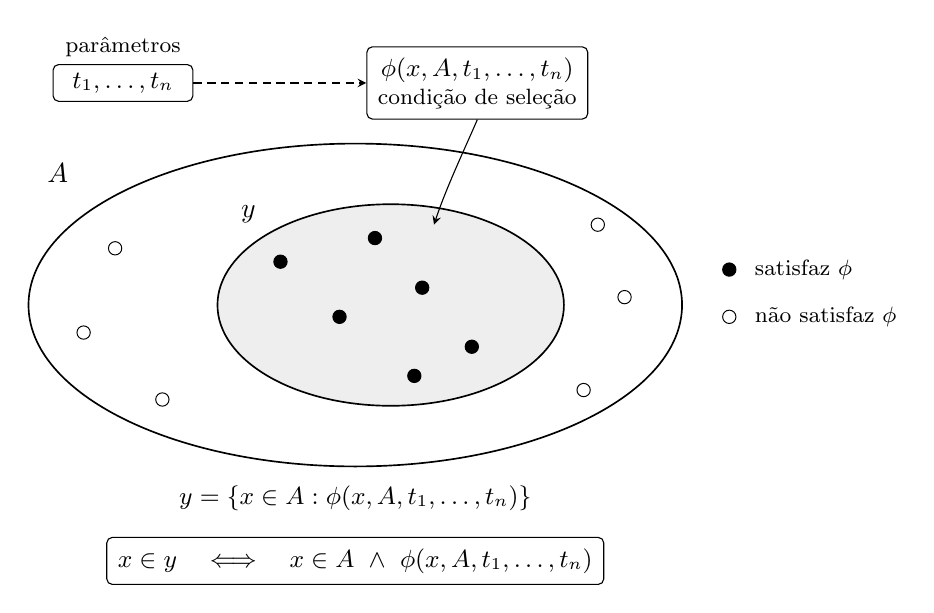
\begin{tikzpicture}[
    x=1cm,
    y=1cm,
    every node/.style={font=\small},
    ponto/.style={circle, draw=black, line width=0.35pt, inner sep=1.7pt},
    selecionado/.style={ponto, fill=black},
    naoSelecionado/.style={ponto, fill=white},
    seta/.style={->, >=stealth, line width=0.4pt},
    caixa/.style={draw=black, rounded corners=2pt, fill=white, inner sep=4pt, align=center}
]

% Conjunto ambiente A:
% oval grande, centralizado na figura, representando o conjunto já dado.
\draw[line width=0.6pt] (0,0) ellipse [x radius=4.15, y radius=2.05];
\node[font=\normalsize] at (-3.78,1.68) {$A$};

% Subconjunto y:
% região sombreada, levemente deslocada para a direita e inteiramente contida em A.
\fill[gray!13] (0.45,0.00) ellipse [x radius=2.20, y radius=1.28];
\draw[line width=0.6pt] (0.45,0.00) ellipse [x radius=2.20, y radius=1.28];
\node[
    fill=white,
    inner sep=1.6pt,
    font=\normalsize,
    anchor=south east
] at (-1.20,0.98) {$y$};

% Elementos de A que não satisfazem phi:
% pontos vazados, todos dentro de A e fora da região sombreada y.
\foreach \p in {(-3.05,0.72),(-3.45,-0.35),(-2.45,-1.20),(3.08,1.02),(3.42,0.10),(2.90,-1.08)}
    \node[naoSelecionado] at \p {};

% Elementos de A que satisfazem phi:
% pontos preenchidos, todos dentro da região sombreada y.
\foreach \p in {(-0.95,0.55),(-0.20,-0.15),(0.25,0.85),(0.85,0.22),(1.48,-0.53),(0.75,-0.90)}
    \node[selecionado] at \p {};

% Parâmetros:
% colocados acima e fora de A. A seta tracejada indica dependência da fórmula,
% não pertinência ao conjunto ambiente.
\node[font=\footnotesize] at (-2.95,3.28) {parâmetros};
\node[caixa, inner xsep=7pt, inner ysep=3pt] (params) at (-2.95,2.82)
    {$t_1,\ldots,t_n$};

% Fórmula de seleção:
% colocada acima de A e alinhada horizontalmente aos parâmetros.
\node[caixa] (cond) at (1.55,2.82)
    {$\phi(x,A,t_1,\ldots,t_n)$\\[-1pt]
     \footnotesize condição de seleção};

\draw[seta, densely dashed] (params.east) -- (cond.west);
\draw[seta] (cond.south) .. controls (1.42,2.05) and (1.15,1.48) .. (1.00,1.02);

% Legenda:
% posicionada à direita da figura principal, fora do oval A,
% para não ser confundida com elementos do conjunto.
\node[selecionado] at (4.75,0.45) {};
\node[anchor=west, align=left, font=\footnotesize] at (4.95,0.45)
    {satisfaz $\phi$};

\node[naoSelecionado] at (4.75,-0.15) {};
\node[anchor=west, align=left, font=\footnotesize] at (4.95,-0.15)
    {não satisfaz $\phi$};

% Identificação do subconjunto separado:
% centralizada abaixo do oval A.
\node[font=\small] at (0,-2.45)
    {$y=\{x\in A:\phi(x,A,t_1,\ldots,t_n)\}$};

% Equivalência característica:
% centralizada abaixo da identificação de y.
\node[caixa, font=\small] at (0,-3.25)
    {$x\in y\quad\Longleftrightarrow\quad x\in A\ \land\ \phi(x,A,t_1,\ldots,t_n)$};

\end{tikzpicture}
\caption{Compreensão como separação: a fórmula $\phi$, com parâmetros $t_1,\ldots,t_n$, seleciona em $A$ os elementos que formam $y\subseteq A$.}
\label{fig:compreensao-separacao}
\end{figure}